\chapter{Dashboard}
\label{chap:dashboard}

The dashboard is the Next.js app. Sign-in is required. The first time the app has no Clerk keys, the sign-in page asks for them and stores them for the API and the web process; keys in the environment take priority. After sign-in the sidebar is the same on every page: Overview, Repositories, Quality, AI providers, and API keys and MCP. A bell in the header lists notifications.

The wireframes in this chapter are drawings of those screens. They show structure, not the visual design of the running app.

\section{Live updates}

The worker writes Postgres first, then publishes on Redis. The API keeps one subscriber and fans events out to browsers.

\begin{figure}[H]
  \centering
  \resizebox{\linewidth}{!}{% Realtime path: Postgres is the source of truth, Redis fans events out over SSE.
\begin{tikzpicture}[x=1cm,y=1cm]
  \node[sys] (worker) at (1.8,2.3) {Worker};
  \node[store] (pg) at (6.3,3.6) {Postgres};
  \node[store] (redis) at (6.3,1.0) {Redis Pub/Sub};
  \node[sys] (api) at (10.5,2.3) {Core API\\SSE};
  \node[sys] (dash) at (14.0,2.3) {Dashboard};

  \draw[flow] (worker.north east) -- node[flabel, above, sloped] {write first} (pg.west);
  \draw[flow] (worker.south east) -- node[flabel, below, sloped] {then publish} (redis.west);
  \draw[flow] (pg.east) -- (api.north west);
  \draw[flow] (redis.east) -- (api.south west);
  \draw[flow] (api) -- node[flabel, above] {SSE} (dash);

  \node[note, text width=12.2cm, anchor=north west] at (0.15,-0.15) {%
    Channels: \texttt{notify:user:<userId>} for the notification bell, and \texttt{review:<reviewId>} for the pipeline timeline.
    On each reconnect the dashboard reads the database again, and it polls slowly while the stream is down.%
  };
\end{tikzpicture}
}
  \caption{Live updates. The browser uses \code{fetch} for the stream because \code{EventSource} cannot send the Clerk \code{Authorization} header.}
  \label{fig:realtime}
\end{figure}

\code{GET /api/notifications/stream} feeds the bell. \code{GET /api/reviews/:id/stream} feeds the timeline of an open review. The stream sends a ready event on connect and a heartbeat every 25 seconds. When the last listener leaves, the API unsubscribes from that channel. If the stream drops, the page polls slowly and catches up from the database on the next connect.

\section{Landing}

The public page is a dark marketing screen: a short pitch, a link into the dashboard, and the three-step story of connecting a repository, opening a pull request, and receiving inline comments.

\begin{figure}[H]
  \centering
  \resizebox{0.92\linewidth}{!}{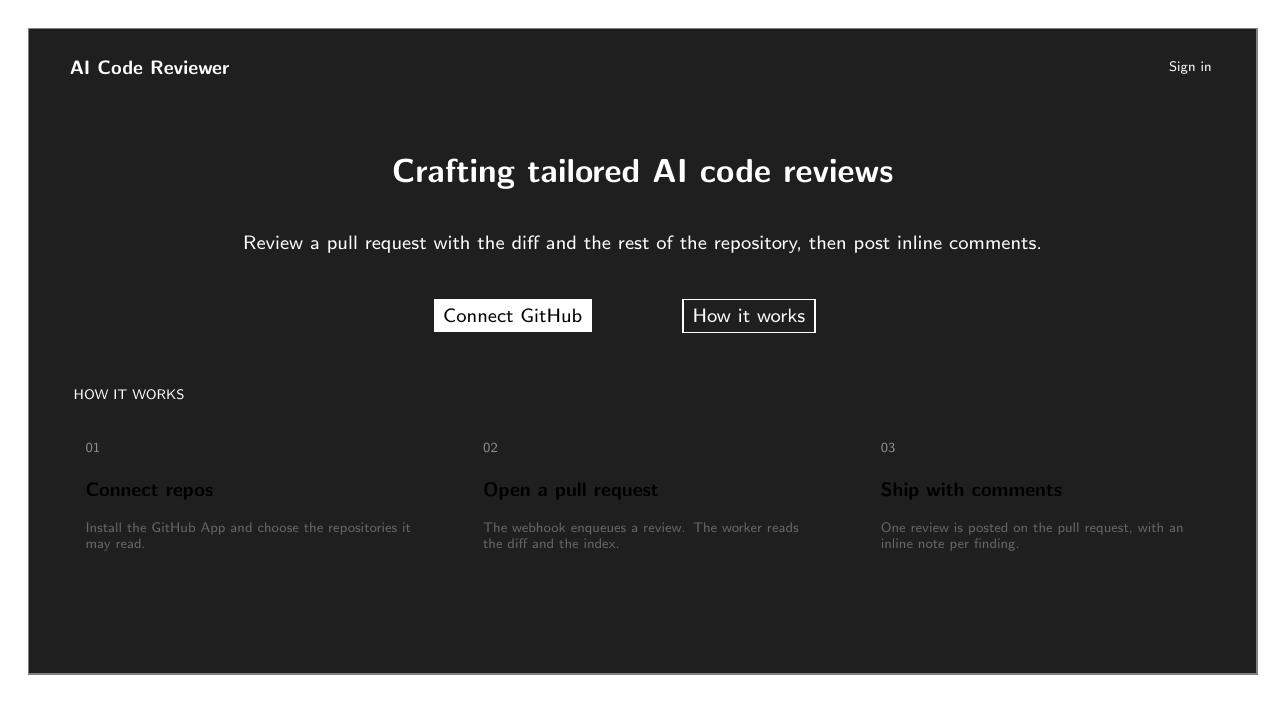
\begin{tikzpicture}[x=1cm,y=1cm]
  \fill[black!88] (0,0) rectangle (15.6,8.2);
  \draw[black!50, line width=0.6pt] (0,0) rectangle (15.6,8.2);

  \node[anchor=west, font=\sffamily\bfseries\scriptsize, text=white] at (0.4,7.7) {AI Code Reviewer};
  \node[anchor=east, font=\sffamily\tiny, text=white!75] at (15.15,7.7) {Sign in};

  \node[align=center, font=\sffamily\bfseries\large, text=white, text width=12cm] at (7.8,6.35)
    {Crafting tailored AI code reviews};
  \node[align=center, font=\sffamily\scriptsize, text=white!65, text width=11cm] at (7.8,5.45)
    {Review a pull request with the diff and the rest of the repository, then post inline comments.};

  \node[fill=white, font=\sffamily\scriptsize, inner sep=3.5pt] at (6.15,4.55) {Connect GitHub};
  \node[draw=white!50, font=\sffamily\scriptsize, text=white, inner sep=3.5pt] at (9.15,4.55) {How it works};

  \node[anchor=west, font=\sffamily\tiny, text=white!50] at (0.45,3.55) {HOW IT WORKS};

  \wfpanel{0.4}{0.4}{4.7}{2.85}
  \node[anchor=north west, font=\sffamily\tiny, text=black!45] at (0.6,3.05) {01};
  \node[anchor=north west, font=\sffamily\bfseries\scriptsize] at (0.6,2.55) {Connect repos};
  \node[anchor=north west, font=\sffamily\tiny, text=black!60, text width=4.2cm] at (0.6,2.05)
    {Install the GitHub App and choose the repositories it may read.};

  \wfpanel{5.45}{0.4}{4.7}{2.85}
  \node[anchor=north west, font=\sffamily\tiny, text=black!45] at (5.65,3.05) {02};
  \node[anchor=north west, font=\sffamily\bfseries\scriptsize] at (5.65,2.55) {Open a pull request};
  \node[anchor=north west, font=\sffamily\tiny, text=black!60, text width=4.2cm] at (5.65,2.05)
    {The webhook enqueues a review. The worker reads the diff and the index.};

  \wfpanel{10.5}{0.4}{4.7}{2.85}
  \node[anchor=north west, font=\sffamily\tiny, text=black!45] at (10.7,3.05) {03};
  \node[anchor=north west, font=\sffamily\bfseries\scriptsize] at (10.7,2.55) {Ship with comments};
  \node[anchor=north west, font=\sffamily\tiny, text=black!60, text width=4.2cm] at (10.7,2.05)
    {One review is posted on the pull request, with an inline note per finding.};
\end{tikzpicture}
}
  \caption{Landing page. Connect GitHub leads to sign-in and then the dashboard.}
  \label{fig:mock-landing}
\end{figure}

\section{Overview}

Three cards read \code{GET /api/stats}: review count, finding count, and how many repositories have reviews enabled. Under them, the latest reviews are merged from each repository, because there is no single ``all reviews'' route.

\begin{figure}[H]
  \centering
  \resizebox{\linewidth}{!}{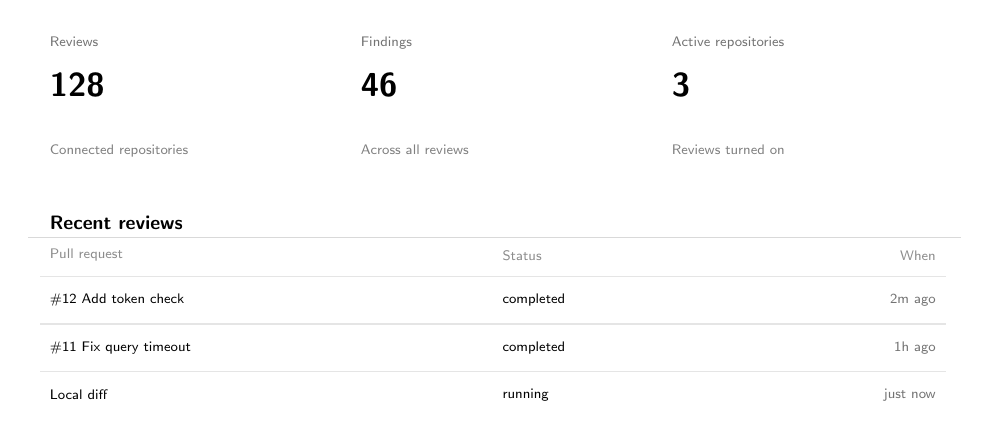
\begin{tikzpicture}[x=1cm,y=1cm]
  \wfchrome{Overview}{7.85}

  \wfpanel{3.40}{5.85}{3.75}{1.85}
  \node[anchor=north west, font=\sffamily\tiny, text=black!55] at (3.55,7.52) {Reviews};
  \node[anchor=north west, font=\sffamily\bfseries\large] at (3.55,7.05) {128};
  \node[anchor=north west, font=\sffamily\tiny, text=black!50] at (3.55,6.15)
    {Connected repositories};

  \wfpanel{7.35}{5.85}{3.75}{1.85}
  \node[anchor=north west, font=\sffamily\tiny, text=black!55] at (7.50,7.52) {Findings};
  \node[anchor=north west, font=\sffamily\bfseries\large] at (7.50,7.05) {46};
  \node[anchor=north west, font=\sffamily\tiny, text=black!50] at (7.50,6.15)
    {Across all reviews};

  \wfpanel{11.30}{5.85}{3.95}{1.85}
  \node[anchor=north west, font=\sffamily\tiny, text=black!55] at (11.45,7.52) {Active repositories};
  \node[anchor=north west, font=\sffamily\bfseries\large] at (11.45,7.05) {3};
  \node[anchor=north west, font=\sffamily\tiny, text=black!50] at (11.45,6.15)
    {Reviews turned on};

  \wfpanel{3.40}{0.35}{11.85}{5.15}
  \node[anchor=north west, font=\sffamily\bfseries\scriptsize] at (3.55,5.25) {Recent reviews};
  \draw[black!15] (3.40,4.85) -- (15.25,4.85);
  \node[anchor=west, font=\sffamily\tiny, text=black!45] at (3.55,4.62) {Pull request};
  \node[anchor=west, font=\sffamily\tiny, text=black!45] at (9.3,4.62) {Status};
  \node[anchor=east, font=\sffamily\tiny, text=black!45] at (15.05,4.62) {When};

  \draw[black!10] (3.55,4.35) -- (15.05,4.35);
  \node[anchor=west, font=\sffamily\tiny] at (3.55,4.05) {\#12  Add token check};
  \node[anchor=west, font=\sffamily\tiny] at (9.3,4.05) {completed};
  \node[anchor=east, font=\sffamily\tiny, text=black!55] at (15.05,4.05) {2m ago};

  \draw[black!10] (3.55,3.75) -- (15.05,3.75);
  \node[anchor=west, font=\sffamily\tiny] at (3.55,3.45) {\#11  Fix query timeout};
  \node[anchor=west, font=\sffamily\tiny] at (9.3,3.45) {completed};
  \node[anchor=east, font=\sffamily\tiny, text=black!55] at (15.05,3.45) {1h ago};

  \draw[black!10] (3.55,3.15) -- (15.05,3.15);
  \node[anchor=west, font=\sffamily\tiny] at (3.55,2.85) {Local diff};
  \node[anchor=west, font=\sffamily\tiny] at (9.3,2.85) {running};
  \node[anchor=east, font=\sffamily\tiny, text=black!55] at (15.05,2.85) {just now};
\end{tikzpicture}
}
  \caption{Overview. A row that is still queued or running is refreshed until it finishes.}
  \label{fig:mock-overview}
\end{figure}

\section{Repositories}

The list is every repository the GitHub App is installed on. The switch turns reviews on or off. Index starts a job and is disabled until an embedding provider is configured. Opening a row goes to that repository.

\begin{figure}[H]
  \centering
  \resizebox{\linewidth}{!}{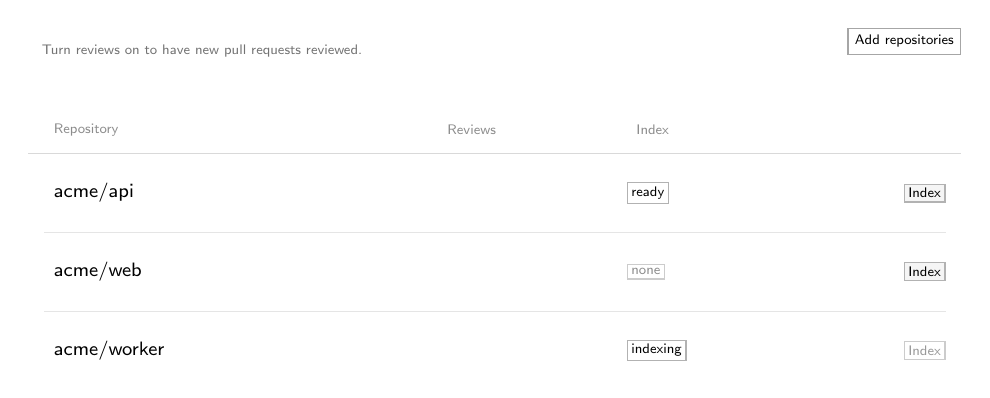
\begin{tikzpicture}[x=1cm,y=1cm]
  \wfchrome{Repositories}{7.25}

  \node[anchor=north west, font=\sffamily\tiny, text=black!55, text width=8.5cm] at (3.45,7.75)
    {Turn reviews on to have new pull requests reviewed.};
  \node[draw=black!35, fill=white, font=\sffamily\tiny, inner sep=2.5pt, anchor=north east] at (15.25,7.85)
    {Add repositories};

  \wfpanel{3.40}{3.20}{11.85}{3.75}
  \node[anchor=west, font=\sffamily\tiny, text=black!45] at (3.60,6.55) {Repository};
  \node[anchor=west, font=\sffamily\tiny, text=black!45] at (8.6,6.55) {Reviews};
  \node[anchor=west, font=\sffamily\tiny, text=black!45] at (11.0,6.55) {Index};
  \draw[black!15] (3.40,6.25) -- (15.25,6.25);

  \node[anchor=west, font=\sffamily\scriptsize] at (3.60,5.75) {acme/api};
  \wfon{8.7}{5.60}
  \node[anchor=west, font=\sffamily\tiny, draw=black!30, inner sep=1.5pt] at (11.0,5.75) {ready};
  \node[draw=black!30, fill=black!4, font=\sffamily\tiny, inner sep=1.5pt, anchor=east] at (15.05,5.75) {Index};

  \draw[black!10] (3.60,5.25) -- (15.05,5.25);
  \node[anchor=west, font=\sffamily\scriptsize] at (3.60,4.75) {acme/web};
  \wfoff{8.7}{4.60}
  \node[anchor=west, font=\sffamily\tiny, draw=black!20, text=black!45, inner sep=1.5pt] at (11.0,4.75) {none};
  \node[draw=black!30, fill=black!4, font=\sffamily\tiny, inner sep=1.5pt, anchor=east] at (15.05,4.75) {Index};

  \draw[black!10] (3.60,4.25) -- (15.05,4.25);
  \node[anchor=west, font=\sffamily\scriptsize] at (3.60,3.75) {acme/worker};
  \wfon{8.7}{3.60}
  \node[anchor=west, font=\sffamily\tiny, draw=black!30, inner sep=1.5pt] at (11.0,3.75) {indexing};
  \node[draw=black!20, text=black!40, font=\sffamily\tiny, inner sep=1.5pt, anchor=east] at (15.05,3.75) {Index};
\end{tikzpicture}
}
  \caption{Repositories. Reviews off means a new pull request is not enqueued.}
  \label{fig:mock-repos}
\end{figure}

\section{One repository}

The repository page has two tabs. Reviews is the history for that repo, with a control to re-run a finished pull-request review. Settings edits strictness, the comment cap, ignored globs (one per line), and custom rules. Each custom rule is a sentence plus a severity. Saved settings apply to the next review, not the one already running.

\begin{figure}[H]
  \centering
  \resizebox{\linewidth}{!}{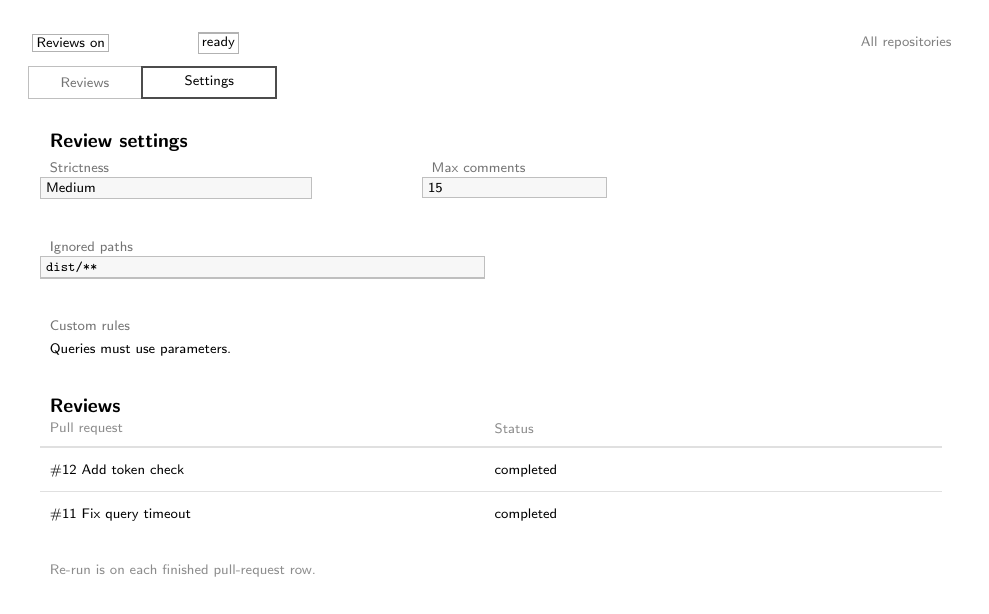
\begin{tikzpicture}[x=1cm,y=1cm]
  \wfchrome{acme/api}{7.25}

  \node[anchor=west, font=\sffamily\tiny, draw=black!30, inner sep=1.4pt] at (3.45,7.55) {Reviews on};
  \node[anchor=west, font=\sffamily\tiny, draw=black!30, inner sep=1.4pt] at (5.55,7.55) {ready};
  \node[anchor=east, font=\sffamily\tiny, text=black!50] at (15.25,7.55) {All repositories};

  % Tabs. Settings is the selected one; the reviews list is drawn below so both are visible.
  \fill[white] (3.40,6.85) rectangle (6.55,7.25);
  \draw[black!25] (3.40,6.85) rectangle (4.85,7.25);
  \draw[black!70, line width=0.7pt] (4.85,6.85) rectangle (6.55,7.25);
  \node[font=\sffamily\tiny, text=black!55] at (4.12,7.05) {Reviews};
  \node[font=\sffamily\tiny] at (5.70,7.05) {Settings};

  \wfpanel{3.40}{3.55}{11.85}{3.15}
  \node[anchor=north west, font=\sffamily\bfseries\scriptsize] at (3.55,6.52) {Review settings};
  \node[anchor=north west, font=\sffamily\tiny, text=black!55] at (3.55,6.15) {Strictness};
  \node[anchor=north west, draw=black!25, fill=black!3, font=\sffamily\tiny, inner sep=2pt, text width=3.3cm] at (3.55,5.85) {Medium};
  \node[anchor=north west, font=\sffamily\tiny, text=black!55] at (8.4,6.15) {Max comments};
  \node[anchor=north west, draw=black!25, fill=black!3, font=\sffamily\tiny, inner sep=2pt, text width=2.2cm] at (8.4,5.85) {15};
  \node[anchor=north west, font=\sffamily\tiny, text=black!55] at (3.55,5.15) {Ignored paths};
  \node[anchor=north west, draw=black!25, fill=black!3, font=\ttfamily\tiny, inner sep=2pt, text width=5.5cm] at (3.55,4.85) {dist/**};
  \node[anchor=north west, font=\sffamily\tiny, text=black!55] at (3.55,4.15) {Custom rules};
  \node[anchor=north west, font=\sffamily\tiny, text width=8cm] at (3.55,3.85) {Queries must use parameters.};

  \wfpanel{3.40}{0.30}{11.85}{3.05}
  \node[anchor=north west, font=\sffamily\bfseries\scriptsize] at (3.55,3.15) {Reviews};
  \node[anchor=west, font=\sffamily\tiny, text=black!45] at (3.55,2.65) {Pull request};
  \node[anchor=west, font=\sffamily\tiny, text=black!45] at (9.2,2.65) {Status};
  \draw[black!12] (3.55,2.42) -- (15.00,2.42);
  \node[anchor=west, font=\sffamily\tiny] at (3.55,2.12) {\#12  Add token check};
  \node[anchor=west, font=\sffamily\tiny] at (9.2,2.12) {completed};
  \draw[black!12] (3.55,1.85) -- (15.00,1.85);
  \node[anchor=west, font=\sffamily\tiny] at (3.55,1.55) {\#11  Fix query timeout};
  \node[anchor=west, font=\sffamily\tiny] at (9.2,1.55) {completed};
  \node[anchor=west, font=\sffamily\tiny, text=black!45] at (3.55,0.85) {Re-run is on each finished pull-request row.};
\end{tikzpicture}
}
  \caption{Repository page. The running app shows one tab at a time. Both are drawn here.}
  \label{fig:mock-repo}
\end{figure}

\section{Review detail}

The title is the pull-request number and title, or ``Local diff review'' when there is no pull request. The timeline is the \code{review\_events} rows. Findings are grouped by file and can be filtered by severity. A finding shows its severity, category, lines, message, and the suggestion when there is one. Re-run is available once the review is no longer queued or running, and only for a pull request.

\begin{figure}[H]
  \centering
  \resizebox{\linewidth}{!}{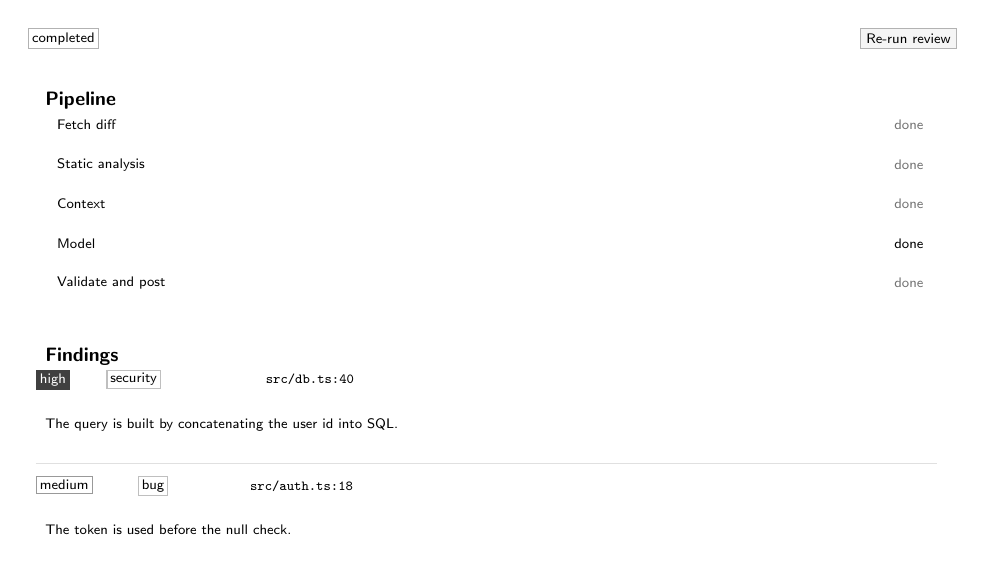
\begin{tikzpicture}[x=1cm,y=1cm]
  \wfchrome{\#12 Add token check}{7.25}

  \node[anchor=west, font=\sffamily\tiny, draw=black!30, inner sep=1.4pt] at (3.45,7.55) {completed};
  \node[anchor=east, draw=black!30, fill=black!4, font=\sffamily\tiny, inner sep=2pt] at (15.25,7.55) {Re-run review};

  \wfpanel{3.40}{4.15}{11.85}{3.05}
  \node[anchor=north west, font=\sffamily\bfseries\scriptsize] at (3.55,7.00) {Pipeline};
  \node[anchor=west, font=\sffamily\tiny] at (3.70,6.45) {Fetch diff};
  \node[anchor=east, font=\sffamily\tiny, text=black!55] at (14.95,6.45) {done};
  \node[anchor=west, font=\sffamily\tiny] at (3.70,5.95) {Static analysis};
  \node[anchor=east, font=\sffamily\tiny, text=black!55] at (14.95,5.95) {done};
  \node[anchor=west, font=\sffamily\tiny] at (3.70,5.45) {Context};
  \node[anchor=east, font=\sffamily\tiny, text=black!55] at (14.95,5.45) {done};
  \node[anchor=west, font=\sffamily\tiny] at (3.70,4.95) {Model};
  \node[anchor=east, font=\sffamily\tiny] at (14.95,4.95) {done};
  \node[anchor=west, font=\sffamily\tiny] at (3.70,4.45) {Validate and post};
  \node[anchor=east, font=\sffamily\tiny, text=black!55] at (14.95,4.45) {done};

  \wfpanel{3.40}{0.30}{11.85}{3.65}
  \node[anchor=north west, font=\sffamily\bfseries\scriptsize] at (3.55,3.75) {Findings};

  \node[anchor=north west, font=\sffamily\tiny, fill=black!75, text=white, inner sep=1.4pt] at (3.55,3.35) {high};
  \node[anchor=west, font=\sffamily\tiny, draw=black!25, inner sep=1.2pt] at (4.45,3.22) {security};
  \node[anchor=west, font=\ttfamily\tiny] at (6.35,3.22) {src/db.ts:40};
  \node[anchor=north west, font=\sffamily\tiny, text width=11cm] at (3.55,2.85)
    {The query is built by concatenating the user id into SQL.};

  \draw[black!12] (3.55,2.15) -- (15.00,2.15);
  \node[anchor=north west, font=\sffamily\tiny, draw=black!40, inner sep=1.4pt] at (3.55,2.00) {medium};
  \node[anchor=west, font=\sffamily\tiny, draw=black!25, inner sep=1.2pt] at (4.85,1.87) {bug};
  \node[anchor=west, font=\ttfamily\tiny] at (6.15,1.87) {src/auth.ts:18};
  \node[anchor=north west, font=\sffamily\tiny, text width=11cm] at (3.55,1.50)
    {The token is used before the null check.};
\end{tikzpicture}
}
  \caption{Review detail. The timeline advances as stage events arrive on the review stream.}
  \label{fig:mock-review}
\end{figure}

\section{Quality}

Quality runs the diffs in \code{evals/} through the same pipeline and scores them: recall (planted issues that were found), precision (findings that hit a planted issue), and false alarms on the clean sample. The page charts those totals and lists each case. Nothing is posted to GitHub.

\section{AI providers}

The page shows which provider will actually run: the main reviewer, the fallback, and the embedding model used for indexing. Keys are split into a free tier and a paid tier, with a link to obtain each key. Saving a key stores it on the user's \code{llm\_settings} row. Clearing the field falls back to the environment value when this user is allowed to use it.

\begin{figure}[H]
  \centering
  \resizebox{\linewidth}{!}{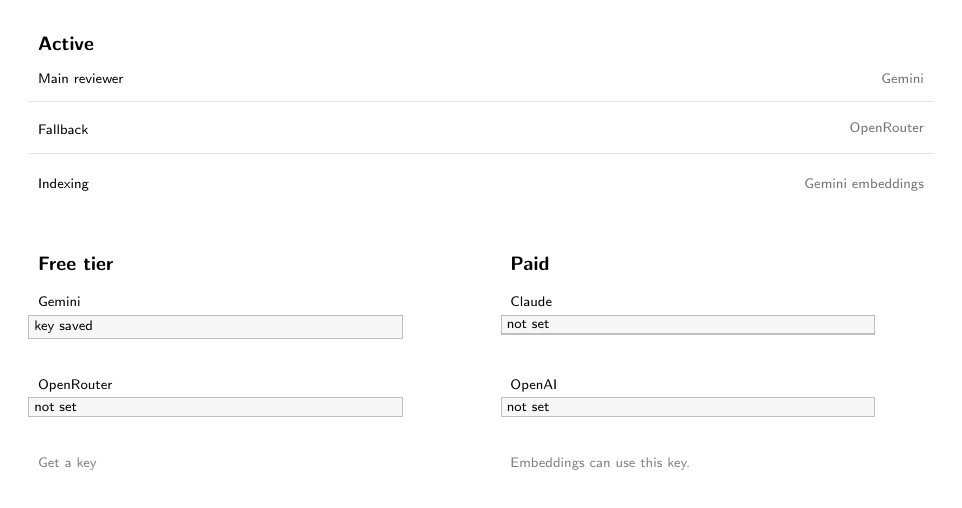
\begin{tikzpicture}[x=1cm,y=1cm]
  \wfchrome{AI providers}{6.05}

  \wfpanel{3.40}{5.15}{11.85}{2.55}
  \node[anchor=north west, font=\sffamily\bfseries\scriptsize] at (3.55,7.50) {Active};
  \node[anchor=west, font=\sffamily\tiny] at (3.55,6.85) {Main reviewer};
  \node[anchor=east, font=\sffamily\tiny, text=black!55] at (15.05,6.85) {Gemini};
  \draw[black!10] (3.55,6.55) -- (15.05,6.55);
  \node[anchor=west, font=\sffamily\tiny] at (3.55,6.20) {Fallback};
  \node[anchor=east, font=\sffamily\tiny, text=black!55] at (15.05,6.20) {OpenRouter};
  \draw[black!10] (3.55,5.90) -- (15.05,5.90);
  \node[anchor=west, font=\sffamily\tiny] at (3.55,5.50) {Indexing};
  \node[anchor=east, font=\sffamily\tiny, text=black!55] at (15.05,5.50) {Gemini embeddings};

  \wfpanel{3.40}{0.35}{5.75}{4.55}
  \node[anchor=north west, font=\sffamily\bfseries\scriptsize] at (3.55,4.70) {Free tier};
  \node[anchor=north west, font=\sffamily\tiny] at (3.55,4.20) {Gemini};
  \node[anchor=north west, draw=black!25, fill=black!3, font=\sffamily\tiny, inner sep=2pt, text width=4.6cm] at (3.55,3.85) {key saved};
  \node[anchor=north west, font=\sffamily\tiny] at (3.55,3.15) {OpenRouter};
  \node[anchor=north west, draw=black!25, fill=black!3, font=\sffamily\tiny, inner sep=2pt, text width=4.6cm] at (3.55,2.80) {not set};
  \node[anchor=north west, font=\sffamily\tiny, text=black!50] at (3.55,2.15) {Get a key};

  \wfpanel{9.40}{0.35}{5.85}{4.55}
  \node[anchor=north west, font=\sffamily\bfseries\scriptsize] at (9.55,4.70) {Paid};
  \node[anchor=north west, font=\sffamily\tiny] at (9.55,4.20) {Claude};
  \node[anchor=north west, draw=black!25, fill=black!3, font=\sffamily\tiny, inner sep=2pt, text width=4.6cm] at (9.55,3.85) {not set};
  \node[anchor=north west, font=\sffamily\tiny] at (9.55,3.15) {OpenAI};
  \node[anchor=north west, draw=black!25, fill=black!3, font=\sffamily\tiny, inner sep=2pt, text width=4.6cm] at (9.55,2.80) {not set};
  \node[anchor=north west, font=\sffamily\tiny, text=black!50] at (9.55,2.15) {Embeddings can use this key.};
\end{tikzpicture}
}
  \caption{AI providers. Indexing stays unavailable until the embeddings row is configured.}
  \label{fig:mock-providers}
\end{figure}

\section{API keys}

Creating a key asks for a name, shows the raw \code{crk\_} value once, and then lists only the prefix, the name, and the last time it was used. The page also shows the command that registers the HTTP MCP server with Claude Code.

\begin{figure}[H]
  \centering
  \resizebox{\linewidth}{!}{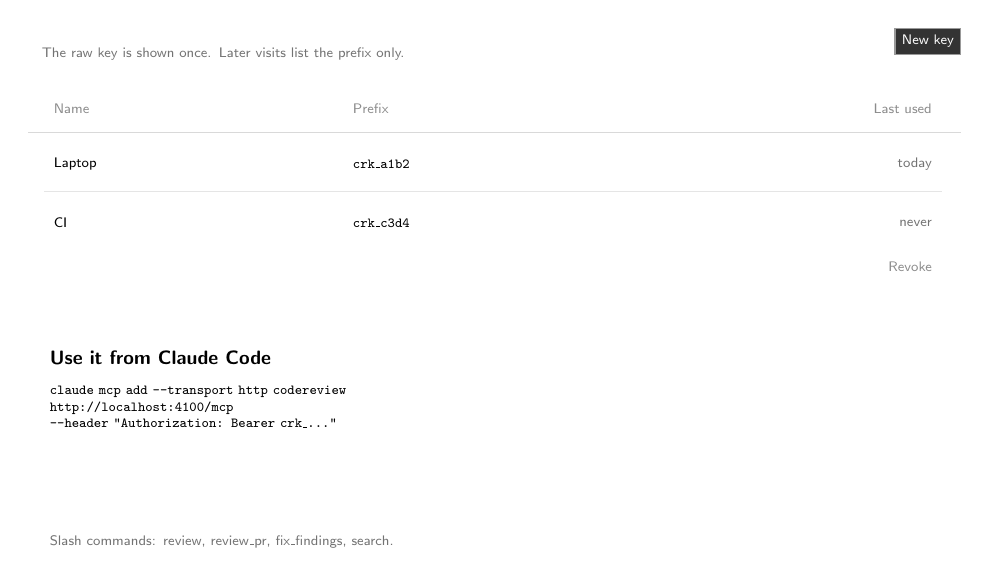
\begin{tikzpicture}[x=1cm,y=1cm]
  \wfchrome{API keys and MCP}{5.45}

  \node[anchor=north west, font=\sffamily\tiny, text=black!55, text width=8.2cm] at (3.45,7.75)
    {The raw key is shown once. Later visits list the prefix only.};
  \node[draw=black!40, fill=black!80, text=white, font=\sffamily\tiny, inner sep=2.5pt, anchor=north east] at (15.25,7.88)
    {New key};

  \wfpanel{3.40}{4.35}{11.85}{2.85}
  \node[anchor=west, font=\sffamily\tiny, text=black!45] at (3.60,6.85) {Name};
  \node[anchor=west, font=\sffamily\tiny, text=black!45] at (7.4,6.85) {Prefix};
  \node[anchor=east, font=\sffamily\tiny, text=black!45] at (15.00,6.85) {Last used};
  \draw[black!15] (3.40,6.55) -- (15.25,6.55);

  \node[anchor=west, font=\sffamily\tiny] at (3.60,6.15) {Laptop};
  \node[anchor=west, font=\ttfamily\tiny] at (7.4,6.15) {crk\_a1b2};
  \node[anchor=east, font=\sffamily\tiny, text=black!55] at (15.00,6.15) {today};
  \draw[black!10] (3.60,5.80) -- (15.00,5.80);

  \node[anchor=west, font=\sffamily\tiny] at (3.60,5.40) {CI};
  \node[anchor=west, font=\ttfamily\tiny] at (7.4,5.40) {crk\_c3d4};
  \node[anchor=east, font=\sffamily\tiny, text=black!55] at (15.00,5.40) {never};
  \node[anchor=east, font=\sffamily\tiny, text=black!45] at (15.00,4.85) {Revoke};

  \wfpanel{3.40}{0.35}{11.85}{3.75}
  \node[anchor=north west, font=\sffamily\bfseries\scriptsize] at (3.55,3.90) {Use it from Claude Code};
  \node[anchor=north west, font=\ttfamily\tiny, text width=11.2cm, align=left] at (3.55,3.45)
    {claude mcp add {-}{-}transport http codereview\\
     http://localhost:4100/mcp\\
     {-}{-}header "Authorization: Bearer crk\_..."};
  \node[anchor=north west, font=\sffamily\tiny, text=black!55, text width=11cm] at (3.55,1.55)
    {Slash commands: review, review\_pr, fix\_findings, search.};
\end{tikzpicture}
}
  \caption{API keys. Revoking a key sets \code{revoked\_at}. The hash cannot be turned back into the secret.}
  \label{fig:mock-keys}
\end{figure}
